\documentclass{beamer}
\usepackage[utf8]{inputenc}
\usepackage[T1]{fontenc}
\usepackage{fancyvrb}
\usepackage{svg}
\usepackage{graphicx}
\usepackage{caption}
\usepackage{hyperref}
%\usepackage{subcaption}
\usepackage{pgfplots}
\pgfplotsset{compat=1.8}
\usepackage{pgfplotstable}
\usepgfplotslibrary{groupplots}

\title{Reinforcement Learning}
\date{WASP Deep Learning}
\author[Agents 47]{The Hitmen --- Agents 47}

\usetheme{wasp}

\graphicspath{{./graphics/}}

\begin{document}

\begin{frame}
  \titlepage
\end{frame}

\begin{frame}{Reinforcement Learning}
  \begin{itemize}
  \item Unlike supervised learning we do not have matching pairs of input and output data to train on.
  \item The agent will instead learn by interacting with the environment. Using some policy the agent performs actions and the environment gives feedback in the form of a reward.\footnote{Image from R. S. Sutton (2017) ``Reinforcement Learning: An Introduction''}
  \begin{figure}
    \centering
    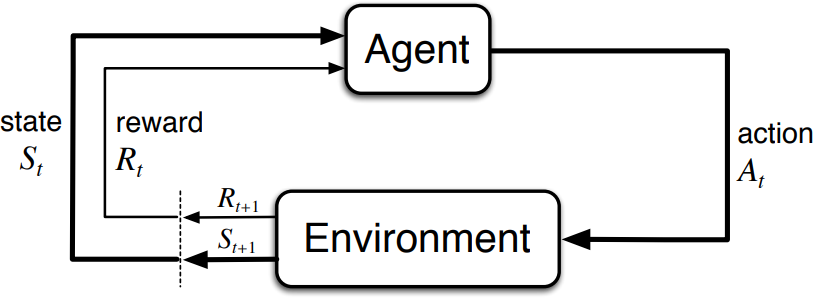
\includegraphics[width=0.8\textwidth]{rl.png}
  \end{figure}
  \end{itemize}
\end{frame}

% Good source: https://en.wikipedia.org/wiki/Q-learning
\begin{frame}{Q-learning}
  \begin{itemize}
  \item In Q-learning we want to, for every given state, find the best action to take, i.e., the action that maximizes all future rewards.
  \item The Q-function $Q(s,a)$ returns the value of performing action $a$ in state $s$ and is updated iteratively:
  \begin{displaymath}
    Q(s_{t},a_{t}) \leftarrow (1-\alpha) \cdot Q(s_{t},a_{t}) + \alpha \cdot  \left( r_{t} + \gamma \cdot \max_a Q(s_{t+1},a) \right)
  \end{displaymath}
  \begin{description}
    \item[$\alpha$ - learning rate] To want extent do we trust the existing $Q(s,a)$ vs. new information.
    \item[$\gamma$ - discount factor] determines the importance of future rewards. A smaller $\gamma$ makes the agent more short-sighted.
  \end{description}
  \end{itemize}
\end{frame}

% Good source: https://youtu.be/lvoHnicueoE?t=894
\begin{frame}{Q-learning cont'd}
  \begin{description}
  \item[Limtation:] We need to define $Q(s,a)$ for every possible state-action pair. This becomes infeasible when the state or action space are of high dimension, e.g., when the state is the pixels in an image.
  \item[Solution:] Train a neural network to approximate $Q(s,a)$. This is called deep Q-learning.
  \end{description}
\end{frame}

% Good source: https://youtu.be/lvoHnicueoE?t=1676
\begin{frame}{Deep Q-learning}
  \begin{description}
  \item[Limtation:] The Q-function can still be complex and difficult to approximate, especially in higher dimensions. Can we find the action to take without involving the Q-function?
  \item[Solution:] Yes, using policy gradients!
  \end{description}
\end{frame}

% Good source: http://karpathy.github.io/2016/05/31/rl/ also https://en.wikipedia.org/wiki/Reinforcement_learning#Direct_policy_search
\begin{frame}{Policy Gradients}
  \begin{itemize}
  \item Construct a mapping from some parameter space to the space of possible policies. Each parameter assignment results in a policy. Optimize over the parameters to find the best policy.
  \item For example, train a neural network to represent our policy:
  \begin{description}
  \item[Input:] Current and possibly previous states.
  \item[Ouput:] The next action to take or a distibution of actions to sample from.
  \end{description}
  In this case, the weights of the network parameterize the policy implemented by the network.
  \end{itemize}
\end{frame}

\begin{frame}{Policy Gradients cont'd}
  \begin{itemize}
  \item The agent performs sets of actions using the current policy.
  \item If the actions result in a large reward they are all determined to be good actions and conversely actions resulting in a small reward are all determined to be bad.
  \item This classification is then used to train the network, making good actions more probable in the future.
  \begin{figure}
    \centering
    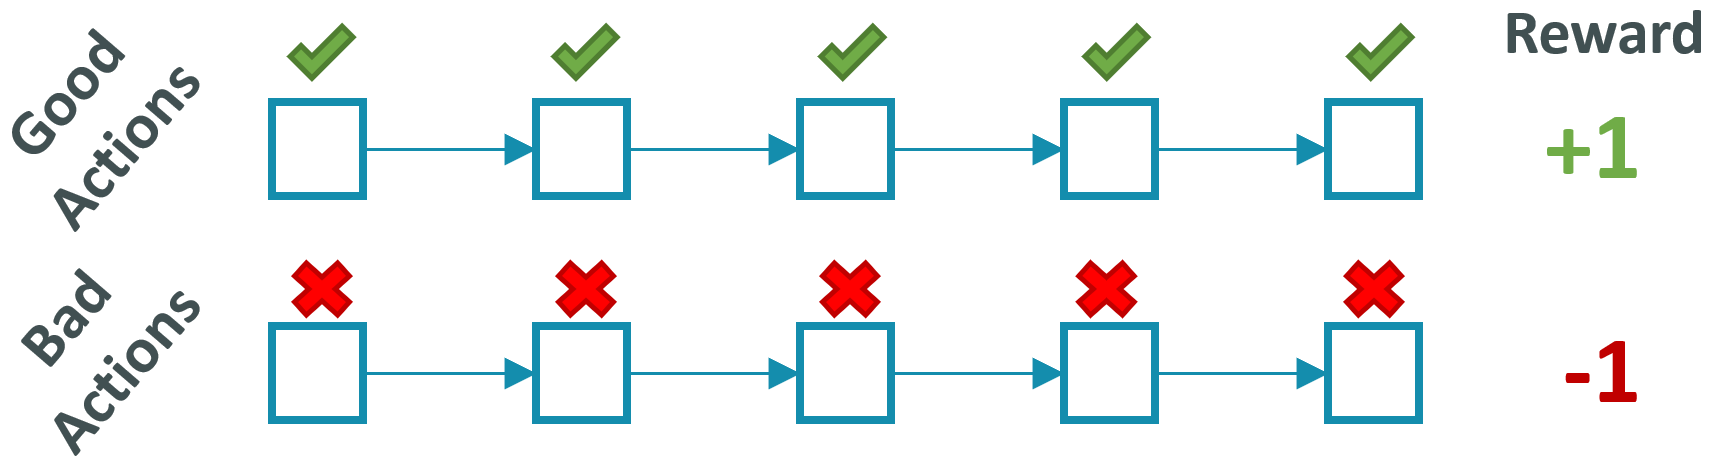
\includegraphics[width=0.85\textwidth]{trajectory_of_actions.png}
  \end{figure}
  \end{itemize}
\end{frame}

% Good source: https://www.youtube.com/watch?v=0Ey02HT_1Ho (sparse rewards)
\begin{frame}{Problems}
  There are some problems with policy gradients and reinforcement learning in general:
  \begin{description}
  \item[Credit assignment:] How do we find out what actions were good or bad in a long trajectory of actions?\\
  Example: what moves caused the agent win a game of chess?
  \item[Sparse reward:] How do we handle sparse rewards?\footnote{See e.g. curiosity-driven exploration and hindsight experience replay.}\\
  Example: starting out with random actions the agent will probably never win a game of chess if no reward is given until the end of the game.
  \end{description}
\end{frame}

% Source: https://youtu.be/lvoHnicueoE?t=2246 (variance reduction)
\begin{frame}{Problems cont'd}
  \begin{description}
  \item[Local minima:] Policy gradients is a local optmization technique and as such we can get stuck on local minima. How do we explore larger policy spaces without getting stuck?
  \item[Slow learning:] Reinforcement learners are slow compared to supervised ones. How can we speed up the learning?\footnote{Init. using supervised learning (e.g. AlphaGo). Also see variance reduction.}
  \end{description}
\end{frame}

\begin{frame}{Resources and references}
  \begin{itemize}
  \item OpenAI Gym (\url{https://gym.openai.com/}) is a toolkit for developing and comparing reinforcement learning algorithms. It provides several environments, e.g., Atari games, simple control problems, MuJuCo and robotics to test in.
  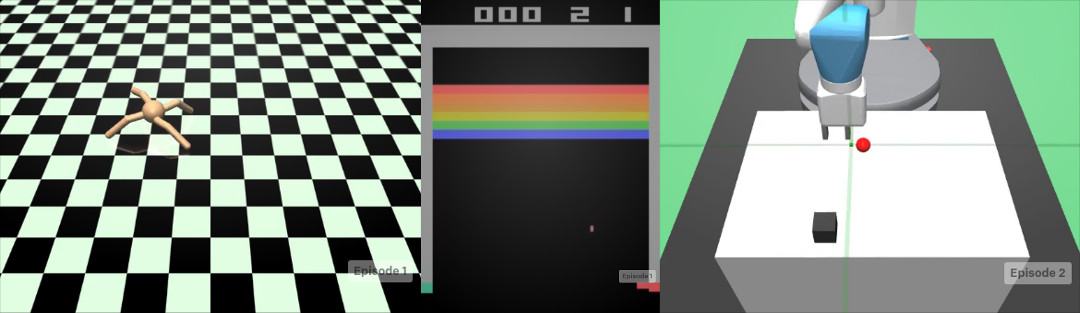
\includegraphics[width=0.8\textwidth]{gym.jpg}
  \item Stanford lecture (\url{https://www.youtube.com/watch?v=lvoHnicueoE})
  \item UCL course (\url{http://www0.cs.ucl.ac.uk/staff/d.silver/web/Teaching.html})
  \end{itemize}
\end{frame}

\end{document}
